\chapter{The Work You've Done}

After the introduction come chapters describing what you've actually done over the course of your research project. 

I haven't done a dissertation so I will just insert a figure, see Figure \ref{myfig}, and a table, see Table \ref{mytab}, so that something appears in my lists of figures and tables. The figure caption also shows how you can give a shortened caption to appear in the list of figures. Make sure that you refer to all figures and tables from the main body of the text and make sure that all text which appears on figures is legible.

\begin{figure}[ht]
\centering
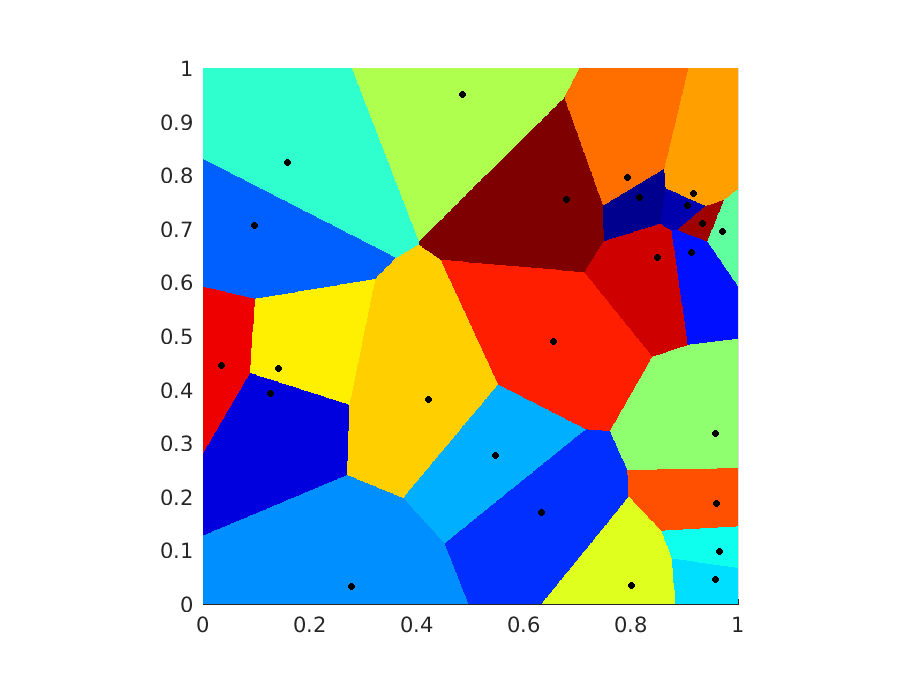
\includegraphics[width=10cm]{voronoi}
\caption[A Voronoi tessellation]{A Voronoi tessellation. The black dots represent 25 randomly chosen nodes in the unit square. The colouring at each other point indicates to which of the nodes it is closest.}
\label{myfig}
\end{figure}


\begin{table}[ht]
\centering
\begin{tabular}{c c c c c c c }
\hline
mesh & $n \_ tri$ & $n \_ nods$ & estimated & actual & estimated &
effectivity \\
& & & current & error & error & index \\
\hline 
1 & 32 & 25 & 1.270 & 0.270 & 0.829 & 3.07 \\
2 & 94 & 59 & 1.131 & 0.131 & 0.413 & 3.16 \\
3 & 201 & 116 & 1.066 & 0.066 & 0.215 & 3.23 \\
4 & 372 & 208 & 1.034 & 0.034 & 0.115 & 3.34 \\ 
5 & 527 & 288 & 1.019 & 0.019 & 0.069 & 3.57 \\ 
6 & 720 & 391 & 1.011 & 0.011 & 0.042 & 3.81 \\
\hline
\end{tabular}
\caption{The triangulations produced by the adaptive finite element method
for the steady state disc electrode problem.}
\label{mytab}
\end{table}


The other thing you need to do is ensure you cite all the relevant materials you have used. Everything that appears in the References should have been cited in the text (if you use BibTeX it's hard not to do this). There are a variety of types of work you might wish to cite, for example a book \cite{abr70}, a journal article \cite{ack77}, a thesis \cite{aldthesis}, work in a collection \cite{bec98} or a conference proceedings \cite{elm92}, or perhaps a technical report \cite{bec99}. In all cases be sure to give enough detail of the reference to allow the reader to find it. If you cite webpages be sure to list the date accessed in the references as in the entry for \cite{strunk}.

You might also like to insert a bullet point list. For this you can decrease the spaces between the bullet points using the itemsep command, see below:
\begin{itemize}
\setlength\itemsep{0em}
\item Item 1
\item Item 2
\item Item 3
\end{itemize}

It can be nice to end each chapter with a brief comment about what you have achieved in that chapter and linking to the next chapter. For example you could say that you have looked at the stability and convergence rates of a numerical scheme in this chapter. In the next chapter you will use the scheme to solve a given problem.